\chapter{Project Cost Management}

Cost management is concerned with estimating, job control and data collection. The following are some techniques which are used to generate outputs such as cost management plans and cost requirements are as follows. 
\begin{enumerate}
\item Plan Cost Management
\item Estimate Costs
\item Determine Budget
\item Control Costs
\end{enumerate}

\section{Planning Cost Management}

Planning for cost management is a important part of cost management. Planning cost from the beginning will ensure accurate time and cost estimates. Expert judgement and experience is essential when managing and controlling project costs through a Cost Management Plan and Project Charters. 

A Cost Management Plan includes:
\begin{enumerate}
\item Units of measure
\item level of precision 
\item level of accuracy
\item Organisational procedures link
\item Control thresholds
\item Rule of performance measurement
\item Reporting formats
\item Process descriptions
\item Additional details
\end{enumerate}

\section{Budgeting}

When estimating cost in a project all risks and environmental and organizational process must be considered. A scope baseline is used to determine and prevent scope creep. An accurate and complete project scope statement, work breakdown structure and WBS dictionary are used to determine the project baseline.

We developed a project cost estimate through an application called COCOMO. The following is an image of the estimate using recent typical salary statistics 
found.

\begin{figure}[H]
\begin{center}
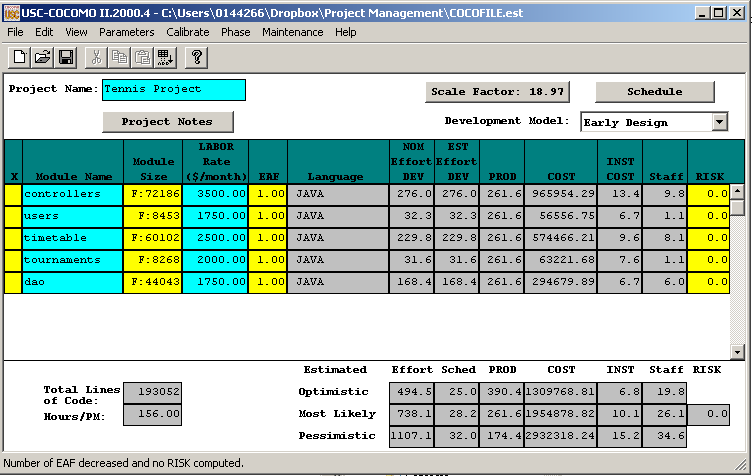
\includegraphics[width=14cm]{cocopre.png}
\end{center}
\caption{COCOMO Early Design}
\label{fig:letter}
\end{figure}

\begin{figure}[H]
\begin{center}
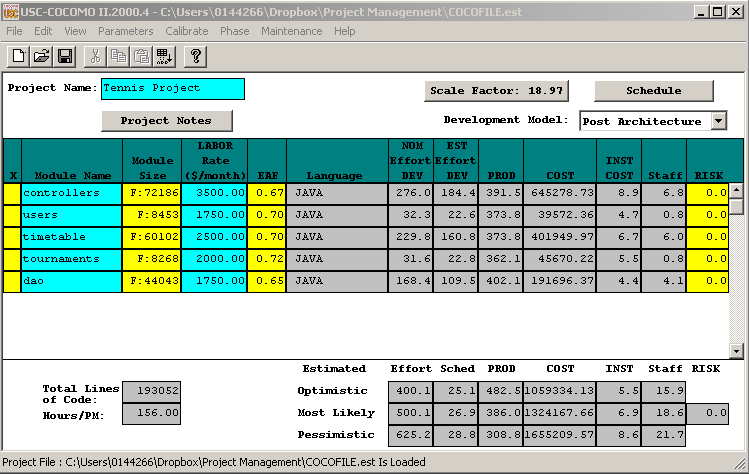
\includegraphics[width=14cm]{cocopost.png}
\end{center}
\caption{COCOMO Post Architecture }
\label{fig:letter}
\end{figure}

The key attribute that we focused on as a cost factor was re-usability. This is concerned with creating a more generic design of software, more elaborate documentation, and more extensive testing to ensure components are ready for use in other applications.

\begin{figure}[H]
\begin{center}
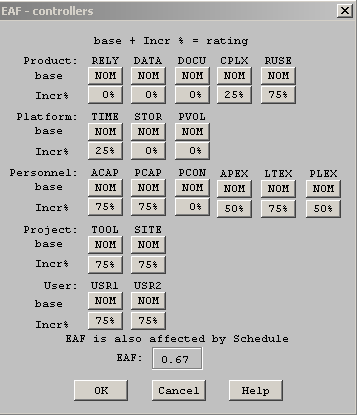
\includegraphics[width=10cm]{coco.png}
\end{center}
\caption{COCOMO Cost Weighting }
\label{fig:letter}
\end{figure}

\begin{enumerate}
\item RELY
\begin{itemize}
\item "This is the measure of the extent to which the software must perform its intended function over a period of time. If the effect of a software failure is only slight inconvenience then RELY is low. If a failure would risk human life then RELY is very high." \parencite{coco}. Within this project, reliability was not especially important and was given a low value.
\end{itemize}
\item DATA
\begin{itemize}
\item "This measure attempts to capture the affect large data requirements have on product development. The rating is determined by calculating D/P. The reason the size of the database is important to consider it because of the effort required to generate the test data that will be used to exercise the program." \parencite{coco}. The database requirements for this project were not massive, so this was given a low ranking.
\end{itemize}
\item DOCU
\begin{itemize}
\item "The rating scale for the DOCU cost driver is evaluated in terms of the suitability of the project's documentation to its life-cycle needs. The rating scale goes from Very Low (many life-cycle needs uncovered) to Very High (very excessive for life-cycle needs)." This is slow as a lot of the factors, such as security of the application, are supported by the frameworks chosen.
\end{itemize}
\item CPLX
\begin{itemize}
\item "Complexity is divided into five areas: control operations, computational operations, device-dependent operations, data management operations, and user interface management operations. Select the area or combination of areas that characterize the product or a sub-system of the product. The complexity rating is the subjective weighted average of these areas." \parencite{coco}. Complexity was adjusted upwards due to the interactions between modules. This was helped by the use of a service layer.
\end{itemize}
\item RUSE
\begin{itemize}
\item "This cost driver accounts for the additional effort needed to construct components intended for reuse on the current or future projects. This effort is consumed with creating more generic design of software, more elaborate documentation, and more extensive testing to ensure components are ready for use in other applications." \parencite{coco}. This was a risk within the project, and the attempt to create a generic solution that could be reused instead of a specific site affected the project costs significantly. 
\end{itemize}
\item TIME
\begin{itemize}
\item "This is a measure of the execution time constraint imposed upon a software system. The rating is expressed in terms of the percentage of available execution time expected to be used by the system or subsystem consuming the execution time resource. The rating ranges from nominal, less than 50\% of the execution time resource used, to extra high, 95\% of the execution time resource is consumed." \parencite{coco}.
\end{itemize}
\item STOR
\begin{itemize}
\item "This rating represents the degree of main storage constraint imposed on a software system or subsystem" \parencite{coco}. This was not deemed to be important due the the cost of increasing memory, storage and processor speed for an application. While optimization is important, this attribute was determined at a much different time in the development industry. 
\end{itemize}
\item PVOL
\begin{itemize}
\item ""Platform" is used here to mean the complex of hardware and software (OS, DBMS, etc.) the software product calls on to perform its tasks. This rating ranges from low, where there is a major change every 12 months, to very high, where there is a major change every two weeks." \parencite{coco}. This is not as important as the application should run with the current version of the framework for a significant amount of time. Updating the frameworks may actually increase development time due to changes introduced. 
\end{itemize}
\item ACAP
\begin{itemize}
\item This is the ability of the analyst to design the application. " The major attributes that should be considered in this rating are Analysis and Design ability, efficiency and thoroughness, and the ability to communicate and cooperate" \parencite{coco}
\end{itemize}
\item PCAP
\begin{itemize}
\item This is the capability of the programming ability within the project. "Evaluation should be based on the capability of the programmers as a team rather than as individuals. Major factors which should be considered in the rating are ability, efficiency and thoroughness, and the ability to communicate and cooperate. The experience of the programmer should not be considered here; it is rated with AEXP. A very low rated programmer team is in the 15th percentile and a very high rated programmer team is in the 95th percentile." \parencite{coco} 
\end{itemize}
\item PCON
\begin{itemize}
\item This is the turnover within the development team. "The rating scale for PCON is in terms of the project's annual personnel turnover: from 3\%, very high, to 48\%, very low." \parencite{coco}
\end{itemize}
\item AEPX
\begin{itemize}
\item "This rating is dependent on the level of applications experience of the project team developing the software system or subsystem" \parencite{coco}. This is how much experience that the chosen development team would have with the frameworks (Spring MVC, Hibernate, Tiles) chosen for this project.
\end{itemize}
\item LTEX
\begin{itemize}
\item The is Language and Tool Experience. "This is a measure of the level of programming language and software tool experience of the project team developing the software system or subsystem." \parencite{coco}
\end{itemize}
\item TOOL
\begin{itemize}
\item This is governed by the use of software tools to aid development. "The tool rating ranges from simple edit and code, very low, to integrated lifecycle management tools, very high." \parencite{coco}. Examples are the use of an IDE like Eclipse, and a source control system, like git.
\end{itemize}
\item SITE
\begin{itemize}
\item This is the cost created by the dispersion of staff within multiple sites. "Determining its cost driver rating involves the assessment and averaging of two factors: site collocation (from fully collocated to international distribution) and communication support (from surface mail and some phone access to full interactive multimedia)." \parencite{coco}
\end{itemize}
\end{enumerate}





\section{Realistic Targets}

Tools and techniques used to generate the work breakdown structures include:
\begin{enumerate}
\item Cost Aggregation 
\begin{itemize}
\item WBS are generated by grouping cost estimates into packages and those packages are then grouped into higher levels of the WBS.
\end{itemize}
\item Reserve Analysis
\begin{itemize}
\item It involves both the contingency reserves and the management reserves. 
\end{itemize}
\item Expert Judgement
\begin{itemize}
\item Mathematical models to predict total project cost are used to reconcile with with any funding limitations. A cost baseline,funding requirements and determined expenditures are now generated form the previous processes.
\end{itemize}
\end{enumerate}

\section{Cost Control}

There must be constant updates made to the project cost plans and any changes to the cost baseline must be updated. These changes are done through Cost forecasts and Change Requests and constantly documented and updated. 
Another technique used to measure project performance is Earned Value Management. This technique integrates scope time and cost date which is determined form the baseline. The following information is input into the EVM on a regular basis.

\begin{enumerate}
\item Planned Value(PV)
\item Actual Cost (AC)
\item Earned Value(EV)
\item Schedule Variances (SV)
\item Cost Variance (CV)
\item Schedule Performance Index(SPI)
\item Cost Performance Index(CPI)
\end{enumerate}

\begin{figure} [H]
\begin{center}
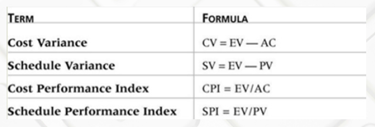
\includegraphics[scale=0.7]{evm.png}
\caption{EVM}
\label{fig:evm}
\end{center}
\end{figure}